% XeLaTeX can use any Mac OS X font. See the setromanfont command below.
% Input to XeLaTeX is full Unicode, so Unicode characters can be typed directly into the source.

% The next lines tell TeXShop to typeset with xelatex, and to open and save the source with Unicode encoding.

%!TEX TS-program = xelatex
%!TEX encoding = UTF-8 Unicode


\documentclass[12pt]{report}


% 宏包配置文件
\usepackage{geometry}                % See geometry.pdf to learn the layout options. There are lots.
\usepackage{graphicx}
\usepackage{xltxtra,xunicode}
\usepackage[CJKnumber,slantfont,boldfont]{xeCJK}
\usepackage{CJKnumb}

\usepackage{titletoc}		% 管理目录格式
\usepackage{titlesec}	% 管理章节标题格式
\usepackage{pstricks}	% 画图
\usepackage{amsfonts}
\usepackage{bm}
\usepackage{booktabs}	% 管理页眉页脚格式
\usepackage{indentfirst}	% 段落首行缩进
\usepackage{enumitem}	% 管理列表项格式
\usepackage{fancyhdr}
\usepackage[numbers,sort&compress]{natbib}	% 管理引用文献格式
\usepackage{CJKpunct}
\usepackage[toc,page,title,titletoc,header]{appendix}
\usepackage{array}
\usepackage{setspace}
\usepackage{amsmath}
\usepackage{amssymb}
\usepackage{fontspec}
\usepackage{unicode-math}		% 数学字体
\usepackage[amsmath,thmmarks,hyperref]{ntheorem}
\usepackage{float}


% 格式文件

\geometry{a4paper}                   % ... or a4paper or a5paper or ... 

% 全文控制
\geometry{left=2.5cm,right=2.5cm,top=2.5cm,bottom=3.5cm}		% 正文与纸张边距
\setlength{\parindent}{24pt}	% 段首行缩进
\linespread{1.5}\selectfont		% 行距设置
%\linespread{1.5}
%\renewcommand{\baselinestretch}{1.38}
% \setlength{\parskip}{1ex}
%\setlength{\parskip}{0.5\baselineskip}
\pagestyle{fancy}
\fancyhead{}
\chead{\xiaowu 河海大学本科毕业论文}  
\setlength{\topmargin}{-0.5cm}
\setlength{\headsep}{0.8cm}

%\setmathfont[math-style=ISO,bold-style=ISO,vargreek-shape=TeX]{TeX Gyre Termes Math}

\setmainfont{Times New Roman}	%缺省英文字体
\defaultfontfeatures{Mapping=tex-text}
\setCJKmainfont{STSong}



\setCJKfamilyfont{heiti}{STHeitiSC-Medium}                                    %黑体  heiti
\newcommand{\heiti}{\CJKfamily{heiti}}                          % 黑体\newcommand{\chuhao}{\fontsize{42pt}
\setCJKfamilyfont{songti}{STSong}                                    %宋体  songti 
\newcommand{\songti}{\CJKfamily{songti}} 
\setCJKfamilyfont{fangsong}{STFangsong} 
\newcommand{\fangsong}{\CJKfamily{fangsong}} 
%\setCJKfamilyfont{menlo}{Menlo} 
%\newcommand{\menlo}{\CJKfamily{menlo}} 
\newfontfamily\menlo{Menlo}
\newfontfamily\consolas{Consolas}

\newcommand{\chuhao}{\fontsize{42pt}{46pt}\selectfont}
\newcommand{\xiaochuhao}{\fontsize{36pt}{40pt}\selectfont}
\newcommand{\yichu}{\fontsize{32pt}{36pt}\selectfont}
\newcommand{\yihao}{\fontsize{26pt}{32pt}\selectfont}
\newcommand{\erhao}{\fontsize{21pt}{24pt}\selectfont}
\newcommand{\xiaoer}{\fontsize{18pt}{20}\selectfont}
\newcommand{\sanhao}{\fontsize{15.75pt}{18pt}\selectfont}
\newcommand{\xiaosan}{\fontsize{15pt}{22.5pt}\selectfont}
\newcommand{\sihao}{\fontsize{14pt}{21pt}\selectfont}
\newcommand{\xiaosi}{\fontsize{12pt}{18pt}\selectfont}
\newcommand{\wuhao}{\fontsize{10.5pt}{13pt}\selectfont}
\newcommand{\xiaowu}{\fontsize{9pt}{11pt}\selectfont}
\newcommand{\liuhao}{\fontsize{7.5pt}{9pt}\selectfont}
\newcommand{\xiaoliuhao}{\fontsize{6.5pt}{7.5pt}\selectfont}
\newcommand{\qihao}{\fontsize{5.5pt}{6.5pt}\selectfont}


\setlength{\parskip}{0pt}% 段距
\newcommand{\mainlineskip}{1.3}% 主行距1.3
\newcommand{\linespacing}[1]{\linespread{#1}\selectfont}% 行距命令

\renewcommand{\contentsname}{\heiti\xiaoer{目\hspace{1em}录}}
\renewcommand\bibname{参考文献}
\renewcommand\thefigure{\thechapter.\arabic{figure}}
\renewcommand{\figurename}{图}
\renewcommand{\theequation}{\arabic{chapter}.\arabic{equation}}
\newcommand{\upcite}[1]{\textsuperscript{\textsuperscript{\cite{#1}}}}






%\DeclareSymbolFont{operators}   {OT1}{ztmcm}{m}{n}
%\DeclareSymbolFont{symbols}     {OMS}{ztmcm}{m}{n}
%\DeclareSymbolFont{bold}        {OT1}{ptm}{bx}{n}
%\DeclareSymbolFont{italic}      {OT1}{ptm}{m}{it}
%\DeclareMathSymbol{\alpha}{0}{letters}{"0B}

%\DeclareSymbolFontAlphabet{\mathrm}{letters}



% 定义目录格式
\titlecontents{chapter}[0pt]{\bfseries\sihao}{第\CJKnumber{\thecontentslabel}章\quad}{}
        {\hspace{0.3em}\titlerule*[4pt]{$\cdot$}\contentspage}
        
\titlecontents{section}[0pt]{\songti\xiaosi}{\thecontentslabel\hspace{0.5em}}{}
        {\hspace{0.3em}\titlerule*[4pt]{$\cdot$}\contentspage}

\titlecontents{subsection}[18pt]{\songti\xiaosi}{\thecontentslabel\hspace{0.5em}}{}
        {\hspace{0.3em}\titlerule*[4pt]{$\cdot$}\contentspage}
              
% 定义章节标题格式
\titleformat{\chapter}[hang]{\centering\xiaoer\heiti}{第\CJKnumber{\thechapter}章}{1em}{}
\titlespacing{\chapter}{0pt}{-3ex  plus .1ex minus .2ex}{3.3ex}

\titleformat{\section}{\sihao\heiti}{\thesection}{1em}{}
\titlespacing{\section}{0pt}{0.5em}{0.5em}

\titleformat{\subsection}{\xiaosi\heiti}{\thesubsection}{1em}{}
\titlespacing{\subsection}{0pt}{0.5em}{0.3em}

\titleformat{\subsubsection}{\xiaosi\heiti}{\thesubsubsection}{1em}{}
\titlespacing{\subsubsection}{0pt}{0.3em}{0pt}

% 定义列表环境
\setlength{\itemindent}{24pt}    %标签缩进量
\setenumerate[1]{itemsep=0pt,partopsep=0pt,parsep=\parskip,topsep=0pt}
\setitemize[1]{itemsep=0pt,partopsep=0pt,parsep=\parskip,topsep=5pt}
\setdescription{itemsep=0pt,partopsep=0pt,parsep=\parskip,topsep=5pt}

\setlength{\bibsep}{0.5ex}  % vertical spacing between references

%\punctstyle{kaiming} 

\renewcommand*{\arraystretch}{0}		% 调整矩阵行间距



\renewcommand{\figurename}{图}
\renewcommand{\tablename}{表}
\renewcommand{\thetable}{\thechapter-\arabic{table}} %修改表格的表头为表2-1
\setlength{\belowcaptionskip}{5pt}

\renewcommand\arraystretch{1}

\theoremstyle{plain} 
\newtheorem{theorem}{\heiti{\hskip 2em 定理}}[chapter]
\newtheorem{definition}{\heiti{\hskip 2em 定义}}[chapter]


\lstset{language=Matlab}
\lstset{breaklines}
\lstset{extendedchars=false}


\begin{document}
\setcounter{secnumdepth}{3}
\xiaosi

\pagenumbering{Roman}
\begin{titlepage}
\makeatletter
\newcommand\dlmu[2][4cm]{\hskip1pt\underline{\hb@xt@ #1{\hss#2\hss}}\hskip3pt}
\makeatother


\newgeometry{top=4.3cm}
\hspace{8.5cm}{\heiti\wuhao 学号\dlmu[3.5cm]{1206010413}}

\hspace{8.5cm}{\heiti\wuhao 年级\dlmu[3.5cm]{12级}}

\vspace{1.3cm}

\begin{center}

\includegraphics[width=12.67cm]{figure/hhu.png}

\vspace{1.3cm}

{\songti\yihao\textbf{本科毕业论文}}

\vspace{1.7cm}

{\heiti\erhao{多核聚类研究}}

\vspace{1.8cm}

\begin{tabular}{p{0.6cm}p{5.5em}@{\extracolsep{0.5em}}lc}
  \vspace{-0.41cm}
  ~ & {\heiti\sanhao 专 \hfill  \hfill 业} & \dlmu[6.08cm]{\songti\xiaosan 计\ 算\ 机\ 科\ 学\ 与\ 技\ 术} & \\
  \vspace{-0.41cm}
  ~ & {\heiti\sanhao 姓 \hfill  \hfill 名} & \dlmu[6.08cm]{\songti\xiaosan 朱\ \ \ 雪\ \ \ 林} & \\
  \vspace{-0.41cm}
  ~ & {\heiti\sanhao 指 \hfill 导 \hfill 教 \hfill 师}& \dlmu[6.08cm]{\songti\xiaosan 王\ 敏、薛\ 晖} & \\
  \vspace{-0.41cm}
  ~ & {\heiti\sanhao 评 \hfill 阅 \hfill 人}& \dlmu[6.08cm]{\songti\xiaosan } & \\
  \vspace{-0.41cm}
\end{tabular}

\vspace{2cm}
{\heiti\sanhao 2 0 1 6 年 4 月} \\
{\heiti\sanhao 中国 \hspace{0.7cm} 南京}
\end{center}

\newpage

\thispagestyle{empty}

\newgeometry{top=4.3cm}

\begin{center}
{\erhao\textbf{BACHELOR'S DEGREE THESIS }}

\vspace{9pt}

{\erhao\textbf{OF HOHAI UNIVERSITY}}

\vspace{3.5cm}

{\erhao\textbf{Multiple Kernel Clustering Research}}

\vspace{4cm}

\begin{table}[htbp]
   \centering
   \renewcommand\arraystretch{1.5}
   \begin{tabular}{l l  l } % Column formatting, @{} suppresses leading/trailing space
   \sihao{College} & \sihao{:} & \sihao{College of Computer and Information} \\
   \sihao{Subject} & \sihao{: }& \sihao{Computer Science and Technology} \\
   \sihao{Name} & \sihao{:} & \sihao{XueLin Zhu} \\
   \sihao{Directed by} & \sihao{:} & \sihao{Min Wang、Hui Xue associate professor} \\
   \end{tabular}
\end{table}

\vspace{1.8cm}
{\xiaoer NANJING\ CHINA}
\end{center}

\newpage
\thispagestyle{empty}
\begin{center}
{\songti\erhao\textbf{郑\ 重\ 声\ 明}}
\end{center}


\noindent\songti\sihao{\hspace{28pt}本人呈交的毕业论文,是在导师的指导下,独立进行研究工作所取得的成果,所有数据、图片资料真实可靠。尽我所知,除文中已经注明引用的内容外,本设计(论文)的研究成果不包含他人享有著作权的内容。对本设计(论文)所涉及的研究工作做出贡献的其他个人和集体,均已在文中以明确的方式标明。本设计(论文)的知识产权归属于培养单位。}

\vspace{1cm}

{\noindent\songti\sihao 本人签名:\dlmu[4cm]{} \hspace{1.5cm} 日期:\dlmu[4cm]{}}

\end{titlepage}

\chapter*{摘\hspace{1em}要}
\addcontentsline{toc}{chapter}{摘\hspace{1em}要}
支持向量机SVM以间隔最大化为学习策略,并引入核技巧实现非线性分类,被公认为目前最好的分类模型。受到间隔最大化学习策略和核技巧在SVM中所取得的卓越性能的启发,本文考虑将间隔最大化学习策略和核技巧从有监督的学习推广到无监督的学习中。

最大间隔聚类MMC的核心思想是首先使用核函数将数据映射到高维的核特征空间,然后寻找一组最优的类标记组合,使得SVM在新的特征空间上训练产生最大的间隔。在此基础上,MMC通过对约束条件进行松弛变换,得到半定规划(SDP)模型。由于最大间隔聚类仅仅依赖于由样本数据生成的核矩阵,因此很容易实现非线性聚类。但最大间隔聚类与其它的核方法一样,核函数的选择将直接决定模型最终性能的好坏,而对于当前特定的任务,如何选择合适的核函数还是一个尚未解决的问题。

多核聚类MKC在此基础上利用有监督和半监督中多核学习的思想,提出对多个核函数进行非负线性组合并得到一个新的基核,再使用这个基核进行训练。MKC在此基础上构造出二阶锥规划(SOCP)模型,并使用割平面算法和凹凸规划对模型进行优化和求解,并同时得到最优的核函数组合、最适当的类标记组合以及最大间隔超平面。

{\heiti 关键字:}聚类;最大间隔聚类;多核聚类;核技巧


\newpage
\chapter*{\textbf{Abstract}}
\addcontentsline{toc}{chapter}{Abstract}
The learning strategy of support vector machine is finding maximum margin hyperplane on training dataset, and it achieves nonlinear classification by using kernel trick. SVM is considered the best classified model at present. Inspired by the outstanding performance of the maximum margin learning strategy and kernel trick in SVM, this paper considers to apply the maximum margin learning strategy and kernel trick from supervised learning to unsupervised  learning. 

The key idea of maximum margin clustering (MMC) is mapping the sample dataset to high-dimensional feature space at first, and then finds a set of optimal class labels so that SVM can find maximum margin by training in new feature space. MMC obtains semidefinite programming model by relaxing constraint condition. MMC is so easy to achieve nonlinear classification by using kernel trick. However, as in other kernel methods, choosing a suitable kernel function is imperative to the success of MMC. But for a current specific task, it is still a unresolved problem to find a suitable kernel function.

Inspired by the works called multiple kernel learning in supervised and semi-supervised leaning, multiple kernel clustering (MKC) proposes a non-negative linear combination of many kernel functions to generate a new base kernel, and then uses this new base kernel to train. MKC constructs second-order cone programing model base on previous idea, using cutting plane algorithm and concave-convex procedure to optimize and solve the model. Finally, it can find the maximum margin hyperplane, the best cluster labeling, and the optimal kernel. 

\textbf{Key words:} Clustering; Maximum margin clustering; Multiple kernel clustering; kernel trick

\clearpage
\addcontentsline{toc}{chapter}{\sihao\bfseries{目\hspace{1em}录}}
\tableofcontents % 自动生成目录


\chapter{绪论}

\pagenumbering{arabic}
\section{研究背景与意义}

聚类是一种无监督的学习,其训练样本的标记信息是未知的,目标是通过对无标记训练样本的学习来揭示数据的内在性质规律,为进一步的数据分析提供基础。聚类试图将数据集中的样本划分为若干个通常是不想交的子集,每个子集称为一个“簇”,使得簇内样本差异很小,簇间样本差异较大。聚类既可以作为一个单独过程,用于寻找数据内在的分布结构,也可作为分类等其他学习任务的前驱过程\upcite{machinelearning}。

聚类是机器学习和数据挖掘领域十分重要的研究课题,尤其在数据挖掘中的应用极为广泛。在商务上,聚类能帮助市场分析人员从客户基本库中发现不同的客户群,并且用购买模式来刻画不同的客户群的特征等;在生物学上,聚类能用于推导植物和动物的分类,对基因进行分类,获得对种群中固有结构的认识等等;在搜索引擎上,聚类能对web上的文档进行分类,挖掘信息等。

但是,传统的聚类只能解决低维数据的聚类问题。由于实际应用中数据十分复杂,比如基因表达数据、图像特征、文档词频数等,其维度能达到成百上千,甚至更高。传统的聚类方法在高维数据集中进行聚类时,主要遇到两个问题:
  \begin{enumerate}[fullwidth,itemindent=24pt]
  \item 高维数据集中存在大量无关的属性,使得在所有维中存在簇的可能性几乎为零;
  \item 高维空间中数据较低维空间中数据分布要稀疏,其中数据间距离几乎相等是普遍现象,而传统聚类方法是基于距离进行聚类的,因此在高维空间中无法基于距离来构建簇。
  \end{enumerate}

\section{聚类方法研究现状}
当前聚类算法主要包括原型聚类、密度聚类和层次聚类等。原型聚类中最简单的当属k均值算法,该算法存在大量的变体,比如k-medoids算法\upcite{kaufman1987clustering}强制原型向量必为训练样本,k-modes算法\upcite{huang1998extensions}可处理离散属性,Fuzzy C-means (FCM) \upcite{bezdek2013pattern}则是“软聚类”算法,允许每个样本以不同程度同时属于多个原型。需要注意的是,k均值类算仅在凸形簇结构上效果很好。最近研究表明,若采用某种Bregman距离,则可显著增强此类算法对更多类型簇结构的适用性\upcite{banerjee2005clustering}。引入核技巧则可得到核k均值算法\upcite{scholkopf1998nonlinear},这与谱聚类\upcite{von2007tutorial}有模切联系。谱聚类可以看作在拉普拉斯特征映射降维后执行k均值聚类。聚类簇数k通常需要用户提供,有一些启发式用于自动确定k\upcite{pelleg2000x},但常用的仍然是基于不同k值多次运行后选取最佳结果。

采用不同方式表征样本分布的紧密程度,可设计出不同的密度聚类算法,除DBSCAN\upcite{ester1996density}外,较常用的还有OPTICS\upcite{ankerst1999optics}、DENCLUE\upcite{hinneburg1998efficient}等。AGNES\upcite{kaufman2009finding}采用自底向上的聚类策略来产生层次聚类结构,与之相反,DIANA\upcite{kaufman2009finding}则采用自顶向下的分拆策略。AGNES和DIANA都不能对已合并或已分拆的聚类簇进行回溯调整,常用的层次聚类如BIRCH\upcite{zhang1996birch}、ROCK\upcite{guha1999rock}等对此进行了改进。

\section{本文的研究动机}
支持向量机以间隔最大化为学习策略,并引入核技巧实现非线性分类器。其优越的分类精度,尤其在文本分类任务中显示出卓越性能\upcite{joachims2000text},被业界公认为最好的分类模型。间隔最大化能保证模型具有较好的泛化能力,核技巧能有效避免“维数灾难”,考虑到间隔最大化和核技巧在分类的卓越性能,那么,将其应用在聚类技术中,取得的性能让人十分期待。

\section{研究目标及内容}
本文的研究目标是:基于间隔最大化学习策略和核技巧的思想,着重研究最大间隔聚类\upcite{mmc} (MMC) 算法和多核聚类\upcite{mkc} (MKC) 算法,详细探讨间隔最大化和核技巧在聚类中所取得的性能。


本文的主要工作内容:
\begin{enumerate}[fullwidth,itemindent=24pt]
  \item 分析间隔最大化学习策略和核技巧的优越之处。从SVM主问题出发以及对偶问题出发研究间隔最大化学习策略和核技巧在SVM中的应用方法。
  \item 分析最大间隔聚类算法原理和模型推导过程。针对分类模型SVM,将其推广到聚类分析中,并通过凸优化技巧进行建模。
  \item 分析多核聚类算法原理和模型推导过程。针对最大间隔聚类算法的局限性,对其进行改进,由单核学习到多核学习。并引入割平面算法和凹凸规划,提高算法的收敛速度。
  \item 针对最大间隔聚类算法和多核聚类算法,使用UCI上的数据集,通过实验来验证算法的性能,并与k均值聚类和谱聚类等算法进行对比。
\end{enumerate}
  
\section{论文结构}
本文共分为六章。第一章介绍了本文工作的研究背景与意义,聚类的研究现状,研究动机以及主要的研究内容和目标;第二章介绍了SVM模型的基本内容,分别从SVM主问题以及对偶问题出发,分析SVM中的间隔最大化学习策略和核技巧的应用,为后续章节提供必要的背景知识;第三章分析了MMC算法的模型推导过程,并提出该算法的局限性;第四章分析了MKC算法的模型推导过程,并提出该算法的优越之处;第五章进行相关实验来验证MMC算法和MKC算法的性能,并与传统的聚类算法进行对比;第六章对本文的工作进行了总结。
\chapter{支持向量机SVM}
SVM是Vapnik\upcite{vladimir1995nature}在1995年提出的一种非常有效的算法,由于其卓绝的分类性能,很快成为机器学习的主流技术。以统计学习理论为基础,SVM提出了间隔 (Margin) 的概念,不但提高了分类精确率,而且保证其训练得到的分类器具有较好的泛化能力。并且在此基础上引入核技巧,在有效解决维数灾难问题的同时,也成为更具实用性的非线性分类模型。本章将重点介绍SVM模型的相关基础知识,分别从SVM的主问题和对偶问题出发,分析其间隔最大化学习策略和核技巧的应用。
\section{SVM模型}
\subsection{硬间隔最大化分类器}
SVM是定义在特征空间上间隔最大的分类器。考虑图\ref{fig:svm}所示的二维二类线性可分的情况:
\begin{figure}[!htbp]
\begin{pspicture}(20,6)
\psline[linewidth=1pt](4,3)(9,1)
\psline[linewidth=1pt](4.345,3.862)(9.345,1.862)
\psline[linewidth=1pt](4.69,4.724)(9.69,2.724)
\psline[linewidth=1pt]{<->}(9,1)(9.69,2.724)
\rput(11.5,1.8){Margin$=\displaystyle\frac{2}{\sqrt{\mathbf{w}^T*\mathbf{w}}}$}
\rput(4,4){$L$}
\rput(3.7,3){$L_1$}
\rput(4.3,4.8){$L_2$}
\psdot[dotscale=1.7](4,2)
\psdot[dotscale=2.7,dotstyle=o](5,2.6)
\psdot[dotscale=1.7](5,2.6)
\psdot[dotscale=1.7](5.8,1.7)
\psdot[dotscale=2.7,dotstyle=o](6.6,1.96)
\psdot[dotscale=1.7](6.6,1.96)
\psdot[dotscale=1.7](7,0.7)
\psdot[dotscale=1.7](8,0.99)
\psdot[dotscale=1.7,dotstyle=o](6.6,4.96)
\psdot[dotscale=1.7,dotstyle=o](5.6,4.96)
\psdot[dotscale=2.7,dotstyle=o](6.4,4.04)
\psdot[dotscale=1.7,dotstyle=o](6.4,4.04)
\psdot[dotscale=1.7,dotstyle=o](7.6,4.06)
\psdot[dotscale=1.7,dotstyle=o](8.3,4.01)
\psdot[dotscale=2.7,dotstyle=o](8.8,3.08)
\psdot[dotscale=1.7,dotstyle=o](8.8,3.08)
\psdot[dotscale=1.7,dotstyle=o](9.6,3.46)
\end{pspicture}
\caption{二维二类分类问题}
\label{fig:svm}
\end{figure}

图中分别使用实心点和空心点表示两类训练样本。其中$L$是将两类样本正确分类的直线,也即分类线,$L_1$和$L_2$ 分别为过各类样本集合中离分类线最近的样本点且平行于分类线$L$的直线,将两类样本之间的间隔定义为直线$L_1$和$L_2$之间的距离。如果分类线$L$不但能够将两类样本完全正确的分开,并且使得两类样本之间的间隔最大,那么就认为分类线$L$是最优分类线。最优分类线不但能最小化经验风险,而且还能使泛化性能最优,从而使得结构风险最小。若将其推广到高维空间,那么最优分类线就变成最优分类面。

考虑两类分类问题,给定训练集$T=\{(\mathbf{x}_i,y_i)\}^m_{i=1}$,其中$\mathbf{x}_i\in X=\mathbf{\mathbb{R}}^n$,$y_i \in \{-1,+1\}$是训练样本所对应的类别标记。则其相应的分类决策函数为$f(x)=\mathrm{sign}(\mathbf{w}^T\mathbf{x}+b)$,分离超平面为:
\begin{align} % requires amsmath; align* for no eq. number
   \mathbf{w}^T\mathbf{x}+b=0
\end{align}

其中,$\mathbf{w}$是权值向量,$b$是偏置。定义超平面$(\mathbf{w},b)$关于训练数据集$T$的函数间隔:
\begin{align} % requires amsmath; align* for no eq. number
   \hat{\gamma}=\min_{1,\cdots,m}y_i(\mathbf{w}^T\mathbf{x}_i+b)
\end{align}

进一步规范化分离超平面的法向量$\mathbf{w}$,也即令$\|\mathbf{w}\|=1$,这时便得到超平面$(\mathbf{w},b)$关于训练数据集$T$的几何间隔:
\begin{align} % requires amsmath; align* for no eq. number
   \gamma=\frac{\hat{\gamma}}{\|\mathbf{w}\|}
   \label{equ:margin} 
\end{align}

那么,求解使得几何间隔最大的分离超平面问题就可以公式化的表示为下面的约束最优化问题:
\begin{equation}
\begin{split} % requires amsmath; align* for no eq. number
   \max_{\mathbf{w},b} \quad & \gamma \\
   s.t. \quad & y_i \left( \frac{\mathbf{w}^T}{\|\mathbf{w}\|}\mathbf{x}_i+\frac{b}{\|\mathbf{w}\|} \right) \ge \gamma, \quad i=1,2,\cdots,m
\end{split}
\end{equation}

考虑函数间隔和几何间隔之间的关系式(\ref{equ:margin}),便可得到线性可分支持向量机学习的最优化问题:
\begin{equation}
\begin{split} % requires amsmath; align* for no eq. number
   \max_{\mathbf{w},b} \quad & \frac{1}{2}\|\mathbf{w}\|^2 \\
   s.t. \quad & y_i(\mathbf{w}^T\mathbf{x}_i+b)-1 \ge 0, \quad i=1,2,\cdots,m
\end{split}
\end{equation}

\subsection{软间隔最大化分类器}
在训练数据线性不可分的情况下,上面的线性可分问题的SVM学习方法是不适用的,这就需要对硬间隔最大化进行松弛,得到软间隔最大化。假设训练数据集$T$中存在一些特异点(outlier),使得训练集$T$是线性不可分的。对其中的每个样本点$(\mathbf{x}_i,y_i)$引进一个松弛变量$\xi_i \ge 0$,使得函数间隔加上松弛变量后大于等于1。同时对每个松弛变量$\xi_i$都要付出一定的代价,便得到线性不可分的线性支持向量机的学习问题:
\begin{equation}
\begin{split} % requires amsmath; align* for no eq. number
   \max_{\mathbf{w},b} \quad & \frac{1}{2}\|\mathbf{w}\|^2+C\sum^m_{i=1}\xi_i \\
   s.t. \quad & y_i(\mathbf{w}^T\mathbf{x}_i+b) \ge 1-\xi_i, \quad i=1,2,\cdots,m \\
   & \xi_i \ge 0, \quad  i=1,2,\cdots,m
\end{split}
\end{equation}

其中,$C > 0$是惩罚参数,用来对错误分类的样本进行惩罚。目标函数包含两层含义:几何间隔尽可能的大,同时使错误分类的样本个数尽可能的小。$C$是调和二者的系数。

\section{对偶问题}
针对上面的软间隔SVM学习问题:
\begin{equation}
\begin{split} % requires amsmath; align* for no eq. number
   \max_{\mathbf{w},b} \quad & \frac{1}{2}\|\mathbf{w}\|^2+C\sum^m_{i=1}\xi_i \\
   s.t. \quad & y_i(\mathbf{w}^T\mathbf{x}_i+b) \ge 1-\xi_i, \quad i=1,2,\cdots,m \\
   & \xi_i \ge 0, \quad  i=1,2,\cdots,m
\end{split}
\label{equ:dualPro}
\end{equation}

求解对偶问题 (\ref{equ:dualPro}) 常用的方法是引入拉格朗日函数:
\begin{align} % requires amsmath; align* for no eq. number
   L(\mathbf{w},b,\mathbf{\xi},\mathbf{\alpha},\mathbf{\mu})=\frac{1}{2}\|\mathbf{w}\|^2+C\sum^{m}_{i=1}\xi_i-\sum^{m}_{i=1}\alpha_i(y_i(\mathbf{w}^T\mathbf{x}_i+b)-1+\xi_i)-\sum^m_{i=1}\mu_i\xi_i \label{equ:Lagrange}
\end{align}

其中$\mathbf{\alpha}$和$\mathbf{\mu}$是拉格朗日乘子,且满足$\mathbf{\xi} \ge 0,\mathbf{\mu} \ge 0$。进一步求$L(\mathbf{w},b,\mathbf{\xi},\mathbf{\alpha},\mathbf{\mu})$对$\mathbf{w},b,\mathbf{\xi}$的极小,即:
\begin{align} % requires amsmath; align* for no eq. number
   \nabla_{\mathbf{w}}L(\mathbf{w},b,\mathbf{\xi},\mathbf{\alpha},\mathbf{\mu})=0 \Rightarrow \mathbf{w}=\sum^m_{i=1}\alpha_iy_i\mathbf{x}_i \label{equ:w} \\
   \nabla_{b}L(\mathbf{w},b,\mathbf{\xi},\mathbf{\alpha},\mathbf{\mu})=0 \Rightarrow \sum^m_{i=1}\alpha_iy_i=0 \label{equ:b} \\
   \nabla_{\xi_i}L(\mathbf{w},b,\mathbf{\xi},\mathbf{\alpha},\mathbf{\mu})=0 \Rightarrow C-\alpha_i-\mu_i=0 \label{equ:xi}
\end{align}

将式(\ref{equ:w})$\sim$(\ref{equ:xi})代入式(\ref{equ:Lagrange})中,则可将SVM主问题转化为下面的对偶问题:
\begin{equation}
\begin{split} % requires amsmath; align* for no eq. number
   \min_{\mathbf{\alpha}} \quad & \frac{1}{2}\sum^m_{i=1}\sum^m_{j=1}\alpha_i\alpha_jy_iy_j(\mathbf{x}_i^T\mathbf{x}_j)-\sum^m_{i=1}\alpha_i \\
   s.t. \quad & \sum^m_{i=1}\alpha_iy_i=0 \\
   & 0 \le \alpha_i \le C \quad  i=1,2,\cdots,m
   \label{equ:dual}
\end{split}
\end{equation}

SVM学习问题最终转化为其对偶问题(\ref{equ:dual})进行求解。常用的优化求解算法主要包括:序列最小最优化方法 (SMO)\upcite{cristianini2000introduction}、选块算法\upcite{cristianini2000introduction}和分解算法\upcite{cristianini2000introduction}。

\section{核技巧}
核技巧是一种用线性分类方法求解非线性分类问题的技术,首先使用一个变换将原空间的数据映射到新空间,然后在新空间里用线性分类学习方法从训练数据中学习分类模型\upcite{李航2012统计学习方法}。

在SVM中应用核技巧,其基本想法就是通过一个非线性变换将输入空间 (欧式空间$\mathbb{R}^n$或离散集合) 对应于一个特征空间 (希尔伯特空间$\mathcal{H}$),使得在输入空间$\mathbb{R}^n$中的超曲面模型对应于特征空间$\mathbb{H}$中的超平面模型 (支持向量机),这样,分类问题的学习任务通过在特征空间中求解线性SVM就可以完成\upcite{李航2012统计学习方法}。下面首先定义核函数的概念:
\begin{definition}
\emph{设$\mathcal{X}$是输入空间 (欧式空间$\mathbb{R}^n$的子集或离散集合),又设$\mathcal{H}$为特征空间 (希尔伯特空间),如果存在一个从$\mathcal{X}$到$\mathcal{H}$的映射:}
\begin{align} % requires amsmath; align* for no eq. number
   \phi(x): \mathcal{X} \to \mathcal{H}
\end{align}

\emph{使得对所有$x,z \in \mathcal{X}$,函数$K(x,z)$满足条件:}
\begin{align} % requires amsmath; align* for no eq. number
   K(x,z) = \phi(x)\cdot \phi(z)
\end{align}

\emph{则称$K(x,z)$为核函数,$\phi(x)$为映射函数,式中$\phi(x)\cdot\phi(z)$为$\phi(x)$与$\phi(z)$的内积\upcite{李航2012统计学习方法}。}
\end{definition}

核技巧的想法是在学习和预测过程中,只显示定义核函数$K(x,z)$,而不是显示定义映射函数$\phi$。观察SVM的对偶学习问题(\ref{equ:dual})的目标函数可以发现$(\mathbf{x}_i^T\mathbf{x}_j)$是两个样本的内积,可以使用核函数$K(\mathbf{x}_i,\mathbf{x}_j)$来代替,便得到非线性SVM的最优化问题:
\begin{equation}
\begin{split} % requires amsmath; align* for no eq. number
   \min_{\mathbf{\alpha}} \quad & \frac{1}{2}\sum^m_{i=1}\sum^m_{j=1}\alpha_i\alpha_jy_iy_jK(\mathbf{x}_i,\mathbf{x}_j)-\sum^m_{i=1}\alpha_i \\
   s.t. \quad & \mathbf{\alpha}^T\mathbf{y}=0 \\
   & 0 \le \alpha_i \le C \quad  i=1,2,\cdots,m
   \label{equ:dual-kernel}
\end{split}
\end{equation}

这等价于将原来的输入空间经过映射函数$\phi$转换到一个新的特征空间,使用特征空间中的内积$\phi(x_i)\cdot\phi(x_j)$来代替输入空间中的内积$(\mathbf{x}_i^T\mathbf{x}_j)$,在训练样本的新的特征空间中学习线性SVM。当映射函数为非线性函数时,学习得到的SVM模型是非线性模型。

核技巧的使用让SVM有效解决了维数灾难问题。此外,根据具体问题的数据样本的分布特点,选择合适的核函数更加有利于向学习问题嵌入其先验知识。

\section{本章小结}
本章主要介绍了 SVM 模型的相关基础知识,分别从SVM的主问题和其对偶问题出发,探讨了模型的构建、约束最优化问题的推导以及核技巧的引入等问题。详细介绍了SVM中的间隔最大化学习策略,以及核技巧的应用方法,为本文后续的研究工作提供了必要的知识背景。鉴于SVM在分类领域所取得的巨大的成功,那么,如果将间隔最大化学习策略和核技巧应用在无监督的聚类学习中,会取得怎样的效果呢{\fangsong ?}受这一灵感的启发,接下来一章开始探讨最大间隔聚类(MMC)算法的原理和模型推导过程。
\setlength{\theorempreskipamount}{6pt}
\setlength{\theorempostskipamount}{-20pt}
\chapter{最大间隔聚类MMC}
由第二章的分析可知,SVM以间隔最大化为学习策略,通过对偶问题引入核技巧,实现高性能的非线性分类模型。因此在本章中,将间隔最大化学习策略和核技巧应用到无监督的聚类学习中,将聚类问题公式化的描述为凸整形规划问题,并对该问题进行松弛变化,得到最终MMC的半定规划模型。

\section{MMC模型}
MMC模型将有监督的软间隔SVM学习过程推广到无监督的学习过程,为无标记的训练数据添加标记,使得添加标记后的训练数据经过软间隔SVM学习后,能够得到最大的间隔。也就是说,给定训练数据$T=\{\mathbf{x}_1,\mathbf{x}_2,\cdots,\mathbf{x}_m\}$,其中$\mathbf{x}_i\in X = \mathbb{R}^m$,MMC将每个样本标记为$y_i\in \{-1,+1\}$,使得这两个正负类别之间的间隔是最大的。

很显然,这样的样本类别标记有$2^m$中组合,因此这个问题在计算上十分困难。但若能将该问题转化为凸整形规划(convex integer program)问题,就有可能得到解析解。在此基础上,通过松弛整形约束将问题转化为半定规划(semidefinite program)问题,通过目前已有的半定规划求解工具包,就能很容易计算得到近似最大间隔的样本类别标记组合。

在进行主要工作之前,需要注意几个问题:
\begin{enumerate}[fullwidth,itemindent=24pt]
  \item 需要在约束中添加类平衡约束。这样做不仅是为了防止所有的样本数据都被分配到相同的类标记中,更重要的是避免受到噪音的干扰,防止模型最终将一个或几个特异样本点分配到一个类中以满足最大间隔的要求。
  \item 由于可能存在一些噪音数据具有相同的类别标记,为了提高MMC的性能,在这里使用软间隔最大化准则。
  \item 尽管理论上将MMC模型推广到多类聚类是可能的,但为了简单起见,这里只关注与二类聚类情况。
  \item 由于SVM中的参数$b$,也就是分类器的偏置,会导致非凸问题的出现,而当前还没找到有效的方法解决这个问题,因此只考虑其次分类器,也即令$b=0$,这样问题(\ref{equ:dual})中的约束$\mathbf{\alpha}^T\mathbf{y}=0$就可以去掉。尽管这样的限制看起来十分严重,但可以通过将训练数据进行中心化来减轻该限制的影响。
  \end{enumerate}

\section{模型推导}
结合上述提到的处理方法,将软间隔SVM对偶问题(\ref{equ:dual-kernel})推广为MMC模型,便得到下面的最优化问题:
\begin{equation}
\begin{split} % requires amsmath; align* for no eq. number
  \min_{\mathbf{y}\in\{-1,+1\}^m} \max_{\mathbf{\alpha}} \quad & 2\mathbf{\alpha}^T\mathbf{e} - \langle K \circ \mathbf{\alpha\alpha}^T,\mathbf{yy}^T \rangle \\
  s.t. \quad & 0\le \mathbf{\alpha} \le C \\
  & -l \le \mathbf{e}^T\mathbf{y} \le l 
  \label{equ:MMC-origin}
\end{split}
\end{equation}

其中,$K$表示由特征向量$\Phi=[\phi(\mathbf{x}_1),\cdots,\phi(\mathbf{x}_m)]$的内积得到$m\times m$的核矩阵,即$K=\Phi^T\Phi$,$k_{ij}=\phi(\mathbf{x}_i)^T\phi(\mathbf{x}_j)$,$\mathbf{e}$表示全1的向量。令$A \circ B$表示矩阵的分量乘法,$\langle A,B \rangle = \sum_{ij}a_{ij}b_{ij}$。约束$-l \le \mathbf{e}^T\mathbf{y} \le l $表示类平衡约束。
由于最优化问题(\ref{equ:MMC-origin})的目标函数不是凸函数,因此无法使用有效的算法去解决。实际上,为了能有效的求解最优化问题(\ref{equ:MMC-origin}),需要下面两个步骤:

(1)重新描述最优化问题(\ref{equ:MMC-origin}),记类标记核矩阵$M=\mathbf{yy}^T$。这样目标函数变成在关于$M$的线性函数上求最大值,因此目标函数是凸函数。这样虽然保证了目标函数具有凸性,但同时也产生了非凸约束$M=\mathbf{yy}^T$。因此必须寻找一种方法来约束$M$,从而保证$M=\mathbf{yy}^T$。

(2)添加一系列的线性约束条件来约束$M$,从而保证$M=\mathbf{yy}^T$。注意到对于任意的$y\in \{-1,+1\}^m$,$M=\mathbf{yy}^T$一定有:
\begin{equation*}
m_{ij} \quad = \quad \left\{
\begin{aligned}
1 \quad & \mathrm{if}\ y_i = y_j \\
-1 \quad & \mathrm{if}\ y_i \neq y_j
\end{aligned}
\right.
\end{equation*}

因此$M$具有传递性、自反性和对称性,并且$M$中有且仅有两种相等的类标记。考虑到这两个性质,下面通过添加一系列线性约束条件来满足这些要求:
\begin{equation*}
\begin{split}
& \mathcal{L}_1:\quad m_{ii}=1;m_{ij}=m_{ji};m_ik\ge m_{ij}+m_{jk}-1;\quad \forall_{ijk} \\
& \mathcal{L}_2:\quad m_{jk} \ge -m_{ij} - m_{ik} - 1; \quad \forall_{ijk} \\
& \mathcal{L}_3:\quad \sum_im_{ij} \le m-2; \quad \forall_j \\
\end{split}
\end{equation*}

这些关于$M$线性约束能够满足条件$M=\mathbf{yy}^T$。最后添加约束:
\begin{equation*}
\begin{split}
\mathcal{L}_4:\quad -l \le \sum_im_{ij} \le l; \quad \forall_j \\
\end{split}
\end{equation*}

来替换类平衡约束,同时这个约束也能满足$\mathcal{L}_3$。

经过上述两个步骤,问题(\ref{equ:MMC-origin})被重新公式化描述为下面的凸整形规划问题:
\begin{equation}
\begin{split}
\min_{M\in\{-1,+1\}^{m\times m}} \quad & \max_{\mathbf{\alpha}} 2\mathbf{\alpha}^Te-\langle K \circ \mathbf{\alpha}\mathbf{\alpha}^T,M \rangle \\ 
s.t. \quad & 0 \le \mathbf{\alpha} \le C,\mathcal{L}_1,\mathcal{L}_2,\mathcal{L}_4
\label{equ:MMC-CIP}
\end{split}
\end{equation}

但是问题(\ref{equ:MMC-CIP})并不适用,因为凸整形规划问题的计算仍然十分困难。因此,需要进一步松弛整形约束$M$,从而得到连续参数空间上的凸优化问题:
\begin{equation}
\begin{split}
\min_{M\in\{-1,+1\}^{m\times m}} \quad & \max_{\mathbf{\alpha}} 2\mathbf{\alpha}^Te-\langle K \circ \mathbf{\alpha}\mathbf{\alpha}^T,M \rangle \\ 
s.t. \quad & 0 \le \mathbf{\alpha} \le C,\mathcal{L}_1,\mathcal{L}_2,\mathcal{L}_4,M\succeq 0
\label{equ:MMC-CP}
\end{split}
\end{equation}

再应用Schur补引理\upcite{lanckriet2004learning},便能推导得到最终的半定规划问题(推导过程见附录A):
\begin{equation}
\begin{split}
\min_{M,\delta,\mathbf{\mu},\mathbf{\nu}} \quad & \delta \\
s.t. \quad & \mathcal{L}_1,\mathcal{L}_2,\mathcal{L}_4,\mathbf{\mu} \ge 0,\mathbf{\nu} \ge 0, M \succeq 0 \\
&    \left[\begin{matrix}
      M \circ K & \mathbf{e} + \mathbf{\mu} - \mathbf{\nu} \\
      (\mathbf{e} + \mathbf{\mu} - \mathbf{\nu})^T & \delta - 2C\mathbf{v}^T\mathbf{e} \\
   \end{matrix}\right] \succeq 0
   \label{equ:MMC-SDP}
\end{split}
\end{equation}

求解半定规划问题(\ref{equ:MMC-SDP})得到最优的矩阵$M^*$,训练样本的类标记$\mathbf{y}=\sqrt{\mathit{\lambda}}\mathbf{v}$,其中$\mathit{\lambda},\mathbf{v}$分别是矩阵$M^*$最大的特征值和相应的特征向量。

\section{本章小结}
MMC将SVM中间隔最大化学习策略和核技巧推广到无监督的聚类学习中,其最终目标是为无标记的训练数据添加类别标记,使得在该组类别标记下的训练数据经过SVM的训练学习后,能够得到最大的间隔。但是在模型构造的过程中,需要去掉偏置参数$b$以避免非凸问题的出现,并且为了得到SDP问题松弛类标记核矩阵约束,这会导致损失部分参数空间。同时MMC与其它核方法一样,难以选择合适的核函数,这些都对MMC的聚类性能和适用性造成一定的影响。就MMC过程中的非凸整形优化问题而言,目前已经有一些不同的优化方法能够解决这个问题,除了这里提到的SDP,还有替代优化以及割平面算法。针对MMC的局限性和新方法的出现,接下来一章将会介绍使用割平面算法,并引入多核学习的多核聚类算法。
\chapter{多核聚类MKC}
经过上一章的分析,MMC的基本原理和模型推导过程都已经十分清晰。但很容易想到,使用半定规划(SDP)解决凸整形优化问题(\ref{equ:MMC-origin})的过程损失了部分参数空间,使得最终求解的最优类标记与实际的类标记之间有一定的偏差。并且MMC与其它核方法一样,核函数的选择将直接决定模型性能的好坏,但目前如何选择合适的核函数仍然是未解决的问题。针对MMC的适用性,在本章中,受到有监督学习中多核学习工作\upcite{mmkl}的鼓舞,在MMC模型的基础上,引入多核学习的思想得到多核聚类(MKC)。MKC针对MMC中的非凸整形优化问题(\ref{equ:MMC-origin}),使用割平面算法\upcite{zhao2008efficient}和凹凸规划进行求解。最终得到最大间隔超平面、最适当的类标记组合以及最优的核函数组合。

\section{MKC模型}
\subsection{多核学习}
MMC与其它核方法一样,都依赖于将数据样本映射到高维的特征空间。但它们都面临一个核心的问题,对于一个特定的任务,不清楚哪个核函数最适合。因此,最近SVM和其它核方法从一系列性质相同或者不同的核中构造出一个核,而不是使用单一固定的核,这样的工作已经显示出令人激动的结果\upcite{mmkl}。允许数据样本在不同特征空间的映射合并为一个基核,这样带来很大的灵活性。基于这些启发,MKC将MMC的单核学习改进为多核学习,详细的说,MKC考虑将$M$个特征映射$\Phi_1,\cdots,\Phi_M$ (对应于$M$个基核$K_1,\cdots,K_M$)进行非负线性组合,公式化描述如下:
\begin{align} % requires amsmath; align* for no eq. number
   \Phi(\mathbf{x})=\sum^M_{k=1}\beta_k\Phi_k(\mathbf{x})
\end{align}

其中,$\beta_k\ge 0$,并且存在整数$p$,使得$\sum_k\beta^p_k \le 1$。通过同时考虑到超平面参数(权值$\mathbf{w}$和偏置$b$)和权重参数$\beta_k$来优化MMC中的目标函数,就能得到最优的MMC特征映射。

\subsection{优化过程}
论文的后面将会看到,原始MKC最优化问题的约束条件数非常之多,难以在有限的时间内求解,因此可以通过割平面法\upcite{kelley1960cutting}求解。通过构造一个可嵌套的、逐渐逼近原始MKC最优化问题的松弛序列,序列中的每个最优化问题都可以看作二阶锥规划(SOCP)\upcite{socp},并能通过凹凸规划(CCCP)\upcite{cccp}来求解。

\section{模型推导}
\subsection{单核最大间隔聚类}
在第三章中已经介绍MMC的核心思想,就是将最大间隔标准从有监督的学习推广到无监督的学习中。在二类聚类情况下,给予数据集:$X=\{\mathbf{x}_1,\cdots,\mathbf{x}_m\}$,MMC的目标是寻找最优的标签集合$\mathbf{y}=\{y_1,\cdots,y_m\}\in\{-1,\,+1\}^m$,使得SVM在数据集$\{(\mathbf{x}_1,y_1),\cdots,(\mathbf{x}_m,y_m)\}$上训练并产生最大间隔。对最优化问题(\ref{equ:MMC-origin})重新公式化描述如下:
\begin{equation}
\begin{split}
\min_{y\in\{\pm1\}^m}\min_{\mathbf{w},b,\mathbf{\xi}} \quad & \frac{1}{2}\mathbf{w}^T\mathbf{w}+\frac{C}{m}\sum^m_{i=1}\xi_i \\
s.t. \quad & \forall i\in\{1,\cdots,m\}: \\
& y_i(\mathbf{w}^T\Phi(\mathbf{x}_i)+b) \ge 1-\xi_i,\xi_i \ge 0,  \\
& -l \le \sum^n_{i=1}y_i \le l.
\label{equ:MKC-singalKernel}
\end{split}
\end{equation}

其中,数据样本$X$被映射到高维特征空间,$\Phi$是线性或非线性特征映射。在支持向量机中,通常是使用其对偶形式进行训练的,借助核方法来隐含使用$\Phi$。$\Phi(\mathbf{x})$可以通过计算相应的核矩阵$K$的乔姆斯基(Cholesky)分解得到,也即$K=\hat{X}\hat{X}^T,\Phi(\mathbf{x}_i)=(\hat{X}_{i,1},\cdots,\hat{X}_{i,m})^T$,或者使用特征分解也能得到相同的结果。

此外,问题(\ref{equ:MKC-singalKernel})中的最后一个约束是类平衡约束,其目的是避免所有的训练样本点都被分配相同的类标签。这里$l > 0$是控制类平衡的常数。

根据最优化问题(\ref{equ:MKC-singalKernel}),单核最大间隔聚类在最大化间隔的同时考虑类标记向量$\mathbf{y}$和分离超平面参数$(\mathbf{w},b)$。未知的二值向量$\mathbf{y}$使最优化问题(\ref{equ:MKC-singalKernel})变成整形规划,比SVM中的二次规划(QP)问题更难解决。然而,根据参考文献\cite{zhao2008efficient},我们能将单核最大间隔聚类问题(\ref{equ:MKC-singalKernel})等价的公式化描述为:
\begin{equation}
\begin{split}
\min_{\mathbf{w},b,\mathbf{\xi}}  \quad  & \frac{1}{2}\mathbf{w}^T\mathbf{w}+\frac{C}{m}\sum^m_{i=1}\xi_i \\
s.t. \quad & \forall i\in\{1,\cdots,m\}:  \\
& \left |\mathbf{w}^T\Phi(\mathbf{x}_i)+b \right | \ge 1-\xi_i,\xi_i \ge 0,  \\
& -l \le \sum^n_{i=1} \left [\mathbf{w}^T\Phi(\mathbf{x}_i)+b \right ] \le l.  
\label{equ:MKC-singalKernelRelax}
\end{split}
\end{equation}

其中,标签向量$\mathbf{y}$由$y_i=\mathrm{sign}(\mathbf{w}^T\phi(\mathbf{x}_i)+b)$计算得到,最后一个约束是松弛类平衡约束。与问题(\ref{equ:MKC-singalKernel})相比,问题(\ref{equ:MKC-singalKernelRelax})更加容易处理。

\subsection{多核最大间隔聚类}
由于对某个特定的问题,核函数的适用性是未知的。因此这里利用多个核函数的非负线性组合构造基核,再将这个基核来代替单核最大间隔聚类中的核函数进行训练。详细的说,就是将输入空间中的每个数据样本$\mathbf{x}_i$通过$M$个映射$\Phi_k:\mathbf{x}\mapsto \Phi(\mathbf{x})\in \mathbb{R}^{D_k},k=1,\cdots,M$转换为$M$个特征向量$\Phi_1(\mathbf{x}_i),\cdots,\Phi_M(\mathbf{x}_i)$。这里$D_k$表示第$k$个特征空间的维度。对于每个特征映射来说,都有一个独立的权值向量$\mathbf{w}_k$。从而得到下面的优化问题,当$M=1$时与问题(\ref{equ:MKC-singalKernelRelax})等价。
\begin{equation}
\begin{split}
\min_{\mathbf{\beta},\mathbf{w},b,\mathbf{\xi}} \quad & \frac{1}{2}\sum^M_{k=1}\beta_k\|\mathbf{w}_k\|^2+\frac{C}{m}\sum^m_{i=1}\xi_i \\
s.t. \quad & \forall i \in \{1,\cdots,m\}:  \\
& \left |\sum^M_{k=1}\beta_k\mathbf{w}_k^T\Phi_k(\mathbf{x}_i)+b\right | \ge 1-\xi_i,\xi_i \le 0,   \\
& \forall k \in \{1,\cdots,M\}:\beta_k \ge 0,   \\
& \sum^M_{k=1}\beta_k^p \le 1,   \\
& -l \le \sum^n_{i=1}\left[\sum^M_{k=1}\beta_k\mathbf{w}_k^T\Phi_k(\mathbf{x}_i)+b\right] \le l 
\label{equ:MKC-MultiKernel}
\end{split}
\end{equation}

其中,权值$\beta_k$是用来规则化$M$个输出函数,权值的非负性约束是为了保证核函数之间的线性组合具有凸性,并且能得到基核是半正定的。此外,这里的$p$是一个正整数,这里设定$p=2$,也就是说,使用$l_2$范数对$\mathbf{\beta}=(\beta_1,\cdots,\beta_M)^T$进行规则化。

从问题(\ref{equ:MKC-MultiKernel})中很容易看到,由于成对的参数$\beta_k$和$\mathbf{w_k}$使得目标函数、第一个约束以及最后一个约束都是非凸的。因此,这里需要对变量作一些调整:
\begin{equation}
\forall k\in\{1,\cdots,M\}:\mathbf{v}_k=\beta_k\mathbf{w}_k. 
\end{equation}

进过上面的转换,得到与问题(\ref{equ:MKC-MultiKernel})等价的多核MMC公式化描述:
\begin{equation}
\begin{split}
\min_{\mathbf{\beta},\mathbf{v},b,\mathbf{\xi}} \quad & \frac{1}{2}\sum^M_{k=1}\frac{\|\mathbf{v}_k\|^2}{\beta_k}+\frac{C}{m}\sum^m_{i=1}\xi_i\\
s.t. \quad & \forall i \in \{1,\cdots,m\}:   \\
& \left |\sum^M_{k=1}\mathbf{v}_k^T\Phi_k(\mathbf{x}_i)+b\right | \ge 1-\xi_i,\xi_i \le 0,   \\
& \forall k \in \{1,\cdots,M\}:\beta_k \ge 0,   \\
& \sum^M_{k=1}\beta_k^p \le 1,   \\
& -l \le \sum^n_{i=1}\left [ \sum^M_{k=1}\mathbf{v}_k^T\Phi_k(\mathbf{x}_i)+b\right ] \le l  
\label{equ:MKC-MKv}
\end{split}
\end{equation}

其中,$\mathbf{v}=(\mathbf{v}_1,\cdots,\mathbf{v}_M)^T$。现在除了第一个约束条件外,其余的约束条件以及目标函数都具有凸性。

\subsection{割平面算法}
问题(\ref{equ:MKC-MKv})中有$m$个松弛变量$\xi_i$,对应于每个数据样本。接下来首先对问题(\ref{equ:MKC-MKv})重新公式化描述,减少松弛变量的数量。
\begin{theorem} 
\rm 多核MMC可以被等价的公式化描述为:
\begin{align}
\min_{\mathbf{\beta},\mathbf{v},b,\xi} \quad & \frac{1}{2}\sum^M_{k=1}\frac{\|\mathbf{v}_k\|^2}{\beta_k}+C\xi  \label{equ:MKC-gpm} \\
\nonumber s.t.  \quad & \forall \mathbf{c}\in \{0,1\}^m:   \\
& \frac{1}{m}\sum^m_{i=1}c_i\left |\sum^M_{k=1}\mathbf{v}_k^T\Phi_k(\mathbf{x}_i)+b\right | \ge \frac{1}{m}\sum^m_{i=1}c_i-\xi,  \label{equ:MKC-gpmCon}\\
\nonumber & \forall k \in \{1,\cdots,M\}:\beta_k \ge 0,   \\
\nonumber & \sum^M_{k=1}\beta_k^p \le 1, \xi \ge 0,  \\
\nonumber & -l \le \sum^m_{i=1}\left[\sum^M_{k=1}\mathbf{v}_k^T\Phi_k(\mathbf{x}_i)+b\right] \le l 
\end{align}
\label{theorem:MKC1}
\end{theorem}

{\CJKfontspec{STHeitiSC-Medium}证明}\hspace{1em}为了简单起见,用OP1表示最优化问题(\ref{equ:MKC-MKv}),用OP2表示最优化问题(\ref{equ:MKC-gpm})。证明理论(\ref{theorem:MKC1})成立等价于证明OP1和OP2有相同的最优目标值和等价的约束条件。详细的说,需要证明对于每个$(\mathbf{v},b,\mathbf{\beta})$,最优的$\xi^*$和$\{\xi^*_1,\cdots,\xi^*_m\}$之间满足$\xi^*=\frac{1}{m}\sum^m_{i=1}\xi^*_i$。这就意味着,当$(\mathbf{v},b,\mathbf{\beta})$固定,$(\mathbf{v},b,\mathbf{\beta},\xi^*)$和$(\mathbf{v},b,\mathbf{\beta},\xi^*_1,\cdots,\xi^*_m)$分别是OP1和OP2的最优解,最终得到相同的目标值。

首先,注意到对于任意的$(\mathbf{v},b,\mathbf{\beta})$,OP1中的每个松弛变量$\xi_i$都能被单独的优化:
\begin{equation}
\xi^*_i=\max\left\{0,1-\left |\sum^M_{k=1}\mathbf{v}_k^T\Phi_k(\mathbf{x}_i)+b \right |\right\}  \label{equ:op}
\end{equation}

对于OP2来说,最优的松弛变量$\xi$是:
\begin{equation}
\xi^*=\max_{c\in\{0,1\}^m}\left\{\frac{1}{m}\sum^m_{i=1}c_i-\frac{1}{m}\sum^m_{i=1}c_i\left |\sum^M_{k=1}\mathbf{v}_k^T\Phi_k(\mathbf{x}_i)+b \right |\right\}
\end{equation}

因为在等式 (\ref{equ:op}) 中$c_i$是互不相关的,因此它们也能被单独的优化:
\begin{equation}
\begin{aligned}
\xi^* & =\sum^m_{i=1}\max_{c_i\in\{0,1\}^m}\left\{\frac{1}{m}c_i-\frac{1}{m}c_i\left |\sum^M_{k=1}\mathbf{v}_k^T\Phi_k(\mathbf{x}_i)+b \right |\right\} \\
& = \frac{1}{m}\sum^m_{i=1}\max\left\{0,1-\left |\sum^M_{k=1}\mathbf{v}_k^T\Phi_k(\mathbf{x}_i)+b \right |\right\} \\
& = \frac{1}{m}\sum^m_{i=1}\xi^*_i.
\end{aligned}
\end{equation}

因此,对于任意的$(\mathbf{v},b,\mathbf{\beta})$,给予最优的$\xi^*$和$\{\xi^*_1,\cdots,\xi^*_m\}$,OP1和OP2有相同的目标值。所以,这两个优化问题最优值是相同的。也就是说,我们能通过求解最优化问题(\ref{equ:MKC-gpm})来得到多核MMC的解。定理\ref{theorem:MKC1} 得证。

在最优化问题(\ref{equ:MKC-gpm})中,松弛变量减少了$m-1$个,所有的非凸约束都共用同一个松弛变量$\xi$,这在很大程度上降低了多核MMC中非凸最优化问题的复杂度。另一方面,方程(\ref{equ:MKC-gpmCon})中约束条件的数量从$m$增加到$2^m$,这种指数级增长十分惊人。然而,割平面算法总能找到整个约束集合的一个小的子集,并且在此约束子集上求解得到的结果仍然能保证足够的精度,从而解决多核MMC问题。详细的说,首先初始化一个空的约束子集$\Omega$,计算在满足约束$\Omega$下问题(\ref{equ:MKC-gpm})的最优解;然后割平面算法会寻找(\ref{equ:MKC-gpmCon})中最违背的约束并添加到约束子集$\Omega$中。通过这种思想,割平面算法构造出一系列逐渐逼近原始多核MMC问题的近似值。如果约束集合(\ref{equ:MKC-gpmCon})中在$\epsilon$范围内没有约束是违背的,那么算法终止。算法1是完整的多核MMC割平面算法。
\begin{table}[htbp]
\centering
 \begin{tabular}{lcl}
  \toprule
  {\CJKfontspec{STHeitiSC-Medium}算法1}\hspace{1em}多核最大间隔聚类的割平面算法 \\
  \midrule
 Input:$M$个特征映射$\Phi_1,\cdots,\Phi_M$,参数$C$,$l$和$\epsilon$,约束子集$\Omega= \phi$ \\
 repeat \\
 \hspace{1em}在当前约束子集$\Omega$下求解问题(\ref{equ:MKC-gpm}),得到$(\mathbf{v},b,\mathbf{\beta})$\\
 \hspace{1em}选择最违背的约束$\mathbf{c}$,令$\Omega = \Omega \cup \{\mathbf{c}\}$\\
 until \\
 \hspace{1em}新选择的约束$\mathbf{c}$违背的程度小于$\epsilon$ \\
  \bottomrule
 \end{tabular}
\end{table}

在上述割平面算法中还存在两个问题:
\begin{enumerate}[fullwidth,itemindent=24pt]
   \item 在给予的约束子集$\Omega$下如何求解问题(\ref{equ:MKC-gpm}){\fangsong ?}
   \item 如何在约束集合(\ref{equ:MKC-gpmCon})中找出最违背的约束{\fangsong ?}
\end{enumerate}

这些将在接下来的两个小节中讨论。

\subsubsection{通过CCCP优化}
在割平面算法的每一轮迭代中,需要在当前的约束子集$\Omega$下求解非凸最优化问题(\ref{equ:MKC-gpm}),从而得到最优的分离超平面。尽管问题(\ref{equ:MKC-gpm})中的目标函数是凸的,但约束并不是凸的,这使得问题很难求解。幸运的是,凹凸规划\upcite{cccp}(CCCP)能解决这类最优化问题。详细的说,问题(\ref{equ:MKC-gpm})中的目标函数是二次的,并且除了第一个约束外所有的约束都是线性的。而且,注意到尽管约束集合(\ref{equ:MKC-gpmCon})中的约束是非凸的,但能够写成两个凸函数的差值:
\begin{equation}
\begin{aligned}
& \forall \mathbf{c} \in \Omega: \\
& \left(\frac{1}{m}\sum^m_{i=1}c_i-\xi\right)-\frac{1}{m}\sum^m_{i=1}c_i\left |\sum^M_{k=1}\mathbf{v}_k^T\Phi_k(\mathbf{x}_i)+b \right | \le 0.
\end{aligned}
\end{equation}

因此,可以通过下面的步骤利用CCCP求解最优化问题(\ref{equ:MKC-gpm})。首先初始化$(\mathbf{v}^{(0)},b^{(0)})$,通过将$\frac{1}{m}\sum^m_{i=1}c_i\left |\sum^M_{k=1}\mathbf{v}_k^T\Phi_k(\mathbf{x}_i)+b \right | $替换为其在$(\mathbf{v}^{(t)},b^{(t)})$处的一阶泰勒展开式,CCCP能够从$(\mathbf{v}^{(t)},b^{(t)})$计算得到$(\mathbf{v}^{(t+1)},b^{(t+1)})$。问题(\ref{equ:MKC-gpm})变成:
\begin{equation}
\begin{split}
\min_{\mathbf{\beta},\mathbf{v},b,\mathbf{\xi}} \quad & \frac{1}{2}\sum^M_{k=1}\frac{\|\mathbf{v}_k\|^2}{\beta_k}+C\xi \\
s.t. \quad & \forall \mathbf{c}\in \Omega: \\
& \frac{1}{m}\sum^m_{i=1}c_i \le \xi + \frac{1}{m}\sum^m_{i=1}c_iz^{(t)}_i \left [\sum^M_{k=1}\mathbf{v}_k^T\Phi_k(\mathbf{x}_i)+b \right ]\\
& \forall k \in \{1,\cdots,M\}:\beta_k \ge 0, \\
& \sum^M_{k=1}\beta_k^2 \le 1, \xi \ge 0,\\
& -l \le \sum^m_{i=1}\left[\sum^M_{k=1}\mathbf{v}_k^T\Phi_k(\mathbf{x}_i)+b\right] \le l
\end{split}
\end{equation}
其中$z^{(t)}_i=\mathrm{sign}(\sum^M_{k=1}\mathbf{v}_k^{(t)T}\Phi_k(\mathbf{x}_i)+b^{(t)})$。引入额外的变量$t_k$作为$\frac{\|\mathbf{v}_k\|^2}{\beta_k}$的上界,我们能将上面的问题公式化描述为二阶锥规划(SOCP)问题:
\begin{equation}
\begin{split}
\min_{\mathbf{\beta},\mathbf{v},b,\mathbf{\xi},\mathbf{t}} \quad & \frac{1}{2}\sum^M_{k=1}t_k+C\xi \\
s.t. \quad & \forall \mathbf{c}\in \Omega: \\
& \frac{1}{m}\sum^m_{i=1}c_i \le \xi + \frac{1}{m}\sum^m_{i=1}c_iz^{(t)}_i \left [\sum^M_{k=1}\mathbf{v}_k^T\Phi_k(\mathbf{x}_i)+b \right ]\\
& \forall k \in \{1,\cdots,M\}: \\
& \left\|\left[\begin{matrix} % or pmatrix or bmatrix or Bmatrix or ...
      2\mathbf{v}_k \\
      t_k-\beta_k \\
   \end{matrix}\right]\right\| \le t_k+\beta_k,
  \beta_k \ge 0, \\
& \sum^M_{k=1}\beta_k^2 \le 1, \xi \ge 0,\\
& -l \le \sum^m_{i=1}\left[\sum^M_{k=1}\mathbf{v}_k^T\Phi_k(\mathbf{x}_i)+b\right] \le l
\label{equ:MKC-SOCP}
\end{split}
\end{equation}

这里应用了一个定理,就是形如$\mathbf{s}^T\mathbf{s}\le xy,\ (x,y\in \mathbb{R}_+,\mathbf{s}\in \mathbb{R}^n)$的双曲线约束能被等价地转换为二阶锥约束\upcite{nesterov1994interior,tsang2006efficient}:
\begin{equation}
\left\|\left[\begin{matrix} % or pmatrix or bmatrix or Bmatrix or ...
      2\mathbf{s} \\
      x-y \\
   \end{matrix}\right]\right\| \le x+y,
\end{equation}

由CCCP可知,SOCP问题求得的解$(\mathbf{v},b,\mathbf{\beta},\xi,\mathbf{t})$将作为$(\mathbf{v}^{(t+1)},b^{(t+1)},\mathbf{\beta},\xi,\mathbf{t})$,然后一直迭代直到收敛为止。算法2总结了在满足约束子集$\Omega$下求解问题(\ref{equ:MKC-SOCP})的方法,检查前后两次迭代之间目标函数的差值是否小于$\alpha\%$ (实验中通常将其设置为0.01)作为其终止条件。
\begin{table}[htbp]
\centering
 \begin{tabular}{lcl}
  \toprule
   {\CJKfontspec{STHeitiSC-Medium}算法2}\hspace{1em}满足约束子集$\Omega$条件下通过CCCP求解问题(\ref{equ:MKC-gpm}) \\
  \midrule
 初始化$(\mathbf{v}^{(0)},b^{(0)})$ \\
 repeat \\
 $\quad$求得$(\mathbf{v}^{(t+1)},b^{(t+1)},\mathbf{\beta},\xi,\mathbf{t})$作为SOCP问题(\ref{equ:MKC-SOCP})的解。\\
 $\quad$令$\mathbf{v}=\mathbf{v}^{(t+1)},b=b^{(t+1)},t=t+1$。 \\
 until \\
 $\quad$满足停止准则。\\
  \bottomrule
 \end{tabular}
\end{table}

\newpage

\subsubsection{最违背的约束}
问题(\ref{equ:MKC-gpm})中最违背的约束很容易定义,其约束的可行性由相应的值$\xi$来度量。因此,最违背的约束条件也就是其相应值$\xi$最大。我们用向量$c$来表示约束集合(\ref{equ:MKC-gpmCon})中的每个约束,因此有下面的定理:
\begin{theorem}
\rm 问题(\ref{equ:MKC-gpm})中最违背的约束可以按下面方式计算:
\begin{equation}
c_i=
\begin{cases}
1 & \mathrm{if}\ \left |\sum^M_{k=1}\mathbf{v}_k^T\Phi_k(\mathbf{x}_i)+b \right | < 1 \\
0 & \mathrm{otherwise}
\end{cases}
\label{equ:MVC}
\end{equation}
\label{theorem:MKC2}
\end{theorem}
\hspace{24pt}{\heiti 证明}\hspace{1em}最违背的约束条件也就是其相应值$\xi$最大,为了满足问题(\ref{equ:MKC-gpm})中所有的约束,最优的$\xi$值计算如下:
\begin{align}
\begin{split}
\xi^* & = \sum^m_{i=1}\max_{c_i\in\{0,1\}}\left\{\frac{1}{m}c_i - \frac{1}{m}c_i\left | \sum^M_{k=1}\mathbf{v}_k^T\Phi_k(\mathbf{x}_i)+b \right | \right \} \\
& = \frac{1}{m}\sum^m_{i=1}\max_{c_i\in\{0,1\}}\left\{ c_i \left [ 1 - \left | \sum^M_{k=1}\mathbf{v}_k^T\Phi_k(\mathbf{x}_i)+b \right | \right ] \right \} 
\end{split}
\end{align}

因此,最违背的约束$c$相应的$\xi^*$能够通过等式(\ref{equ:MVC})获得。

割平面算法在迭代时,会选择在当前超平面参数下最违背的约束并将其添加到约束子集$\Omega$,直到在$\epsilon$范围内没有约束是违背的。此外,$\xi$与问题(\ref{equ:MKC-gpm})中的约束集合的可行性有着直接的对应关系,如果点$(\mathbf{v},b,\mathbf{\beta},\xi)$在精度$\epsilon$内满足所有的约束,也就是说:
\begin{align}
\begin{split}
& \forall \mathbf{c} \in \{0,1\}^n: \\
& \frac{1}{m}\sum^m_{i=1}c_i\left | \sum^M_{k=1}\mathbf{v}_k^T\Phi_k(\mathbf{x}_i)+b \right | \ge \frac{1}{m}\sum^m_{i=1}c_i - (\xi + \epsilon)
\label{equ:feasi}
\end{split}
\end{align}

那么点$(\mathbf{v},b,\mathbf{\beta},\xi+\epsilon)$也是可行的。此外,注意到在问题(\ref{equ:MKC-gpm})的目标函数中,松弛变量$\xi$度量了其聚类损失。因此,可以将所有的训练数据都满足不等式(\ref{equ:feasi})作为算法1的终止条件。

\section{本章小结}
MKC对MMC的局限性进行改进,引入多核学习的思想,使用多个核函数的非负线性组合得到的基核进行训练,并使用割平面算法构造一系列逐渐逼近原始多核MMC问题的序列,并且序列中的每个问题都可以通过CCCP进行求解。MKC最终能在训练数据上寻找到最大间隔超平面、最适合的类标记组合以及最优的核函数组合。
\chapter{实验}
通过前面几章对MMC、MKC模型的分析,本章将使用UCI上的数据集验证模型的性能。所有实验的运行环境是MATLAB 8.6,操作系统为Windows 10,硬件环境为3.4GHz Inter Core i7处理器、8GB内存的PC上。

\section{数据集}
本次实验所使用的数据集全部来自UCI仓库,受计算资源等因素的限制,只选择了digits1v7、ionosphere和ringnorm三个数据集。数据描述如表(\ref{tab:dataset})所示:
\begin{table}[!htbp]
\caption{数据集描述}
\centering
\renewcommand\arraystretch{1.5}
\begin{tabular}{|p{3cm}<{\centering}|p{2cm}<{\centering}|p{2cm}<{\centering}|p{2cm}<{\centering}|}
\hline
数据 & 大小 & 维度 & 类别 \\
\hline 
digits1v7 & 776 & 64 & 2 \\
\hline
ionosphere & 354 & 64 & 2 \\
\hline
ringnorm & 1000 & 20 & 2 \\
\hline
\end{tabular}
\label{tab:dataset}
\end{table} 

\section{聚类精度}
首先,本文从聚类精度来验证MMC和MKC的性能。这里的聚类精度是指在最终的聚类结果中,类标记正确的数据样本个数占总数据样本数的百分比。对于MKC,这里使用了三个核函数,分别是:线性核函数$k_1(\mathbf{x}_1,\mathbf{x}_2)=\mathbf{x}_1^T\mathbf{x}_2$,多项式核函数$k_2(\mathbf{x}_1,\mathbf{x}_2)=(\mathbf{x}_1^T\mathbf{x}_2+1)^d$,高斯核函数$k_3(\mathbf{x}_1,\mathbf{x}_2)=\mathrm{exp}(-(\mathbf{x}_1-\mathbf{x}_2)^T(\mathbf{x}_1-\mathbf{x}_2)/2\sigma)$。使用iterSVM\upcite{zhang2009maximum}运行MMC算法,同时为了方便对比,本文使用k均值聚类和谱聚类作为基准。至于MKC模型中的多个参数,本文采用网格搜索,选择其使得聚类结果最优的一组参数建立模型,待搜索的参数空间见表(\ref{tab:para})。

为了评估聚类精度,本文采用的策略是:首先采用有类标记的数据集,去掉所有的类标记并运行聚类算法,然后将聚类得到的结果与类标记进行对比,计算聚类精度。依据此策略,实验最终运行得到的聚类结果见表(\ref{tab:result})。
\begin{table}[!htbp]
\caption{MKC的参数空间}
\centering
\small
\renewcommand\arraystretch{1.5}
\begin{tabular}{p{1.5cm}<{\centering}|p{12cm}}
\hline
参数 & \hspace{0.5cm}取值空间\\
\hline
$C$ &  \hspace{0.5cm}$2^{-6} \quad 2^{-5} \quad 2^{-4} \quad 2^{-3} \quad 2^{-2} \quad 2^{-1} \quad 2^{0} \quad 2^{1} \quad 2^{2} \quad 2^{3} \quad 2^{4} \quad 2^{5} \quad 2^{6} $\\
\hline
$d$ &  \hspace{0.5cm}$2^{0} \quad 2^{1} \quad 2^{2} \quad 2^{3} \quad 2^{4} \quad 2^{5} \quad 2^{6} \quad 2^{7} \quad 2^{8} \quad 2^{9} \quad 2^{10}$ \\
\hline
$\sigma$ &  \hspace{0.5cm}$0.5 \quad 1 \quad 2 \quad 5 \quad 7 \quad 10 \quad 12 \quad 15 \quad 17 \quad 20 $\\
\hline
\end{tabular}
\label{tab:para}
\end{table} 

\begin{table}[!htbp]
\caption{聚类精度(\%)}
\centering
\small
\renewcommand\arraystretch{1.5}
\begin{tabular}{|p{2cm}<{\centering}|p{1.3cm}<{\centering}|p{1.3cm}<{\centering}|p{1.3cm}<{\centering}|p{1.3cm}<{\centering}|p{1.3cm}<{\centering}|p{1.3cm}<{\centering}|p{1.3cm}<{\centering}|}
\hline
数据 & $K_1$ & $K_2$ & $K_3$ & MKC & iterSVM & KM & PC \\
\hline
digits1v7 & 99.61 & 99.61 & 97.62 & 99.74 & 99.36 & 99.23 & 50.26 \\
\hline
ionosphere & 77.78 & 81.48 & 78.06 & 87.46 & 63.84 & 71.23 & 72.60 \\
\hline
ringnorm & 74.50 & 96.90 & 98.70 & 96.50 & 79.11 & 75.55 & 92.27 \\
\hline
\end{tabular}
\label{tab:result}
\end{table}

从表(\ref{tab:result})可以看出,MKC算法的聚类精度确实比MMC、k均值和谱聚类高。在digits1v7、ionosphere和ringnorm三个数据集中,k均值和谱聚类的精度明显受到数据集内部结构的影响,存在忽高忽低的情况。而MKC相比较k均值和谱聚类而言,其聚类结果更加稳定,而且受到数据集内部结构的影响程度不大。但是从图(\ref{fig:ionosphere-gpm})、(\ref{fig:digits1v7-gpm})和(\ref{fig:ringnorm-gpm})可以看出,MKC算法在割平面迭代过程中,其聚类精度是十分不稳定的。随着迭代次数的增加,其聚类精度呈现出上下跳跃的状态,因此,即使割平面最终收敛,但得到的模型的聚类精度可能并不高。所以本文以割平面过程中使得聚类精度最高的参数生成MKC模型,而非最终迭代终止时的参数。

\begin{figure}[H]
  \centering
  \begin{minipage}[t]{0.45\linewidth}
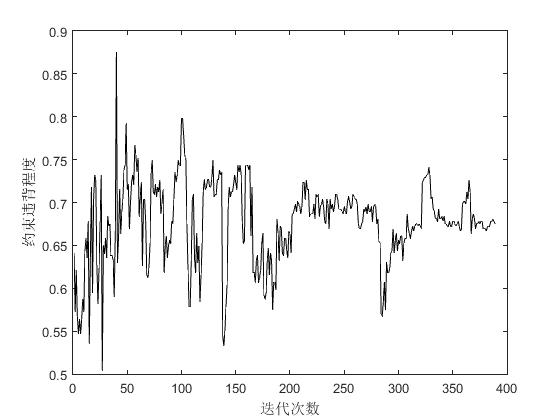
\includegraphics[width=\textwidth]{figure/ionosphere_acc.jpg}
  \caption{ionosphere割平面收敛过程}
  \label{fig:ionosphere-gpm}
  \end{minipage}
  \begin{minipage}[t]{0.45\linewidth}
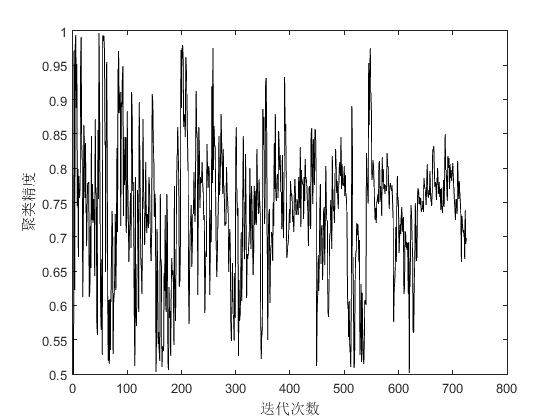
\includegraphics[width=\textwidth]{figure/digits1v7_acc.jpg}
  \caption{digits1v7割平面收敛过程}
  \label{fig:digits1v7-gpm}
  \end{minipage}
  \begin{minipage}[t]{0.45\linewidth}
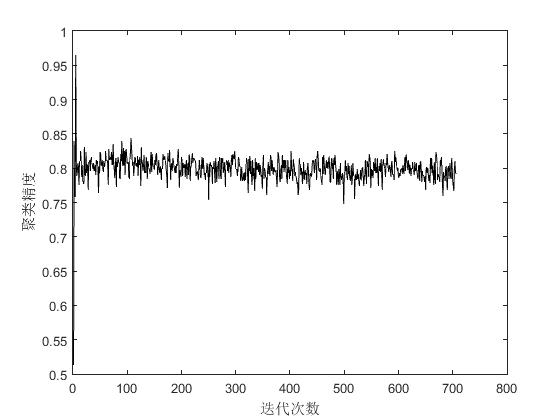
\includegraphics[width=\textwidth]{figure/ringnorm_acc.jpg}
  \caption{ringnorm割平面收敛过程}
  \label{fig:ringnorm-gpm}
  \end{minipage}
\end{figure}



\section{速度}
关于MKC的潜在担忧可能是时间复杂度问题。显然,MKC算法中割平面过程的收敛时间由数据规模和终止条件$\epsilon$共同决定。因此论文从这两个方面进行了相关实验,并将结果进行图形化展示。从图(\ref{fig:time})可以看出,随着数据规模的增大,MKC算法的收敛时间随着终止条件$\epsilon$的减小而迅速增大,甚至在有限的时间内无法收敛。另外从图(\ref{fig:ionosphere-xi})、(\ref{fig:digits1v7-xi})和(\ref{fig:ringnorm-xi})可以看到,MKC的割平面过程收敛十分缓慢,并且存在上下波动的情况,但其总体趋势是下降的,这也符合割平面方法的思想。

\begin{figure}[H]
  \centering
  \begin{minipage}[t]{0.45\linewidth}
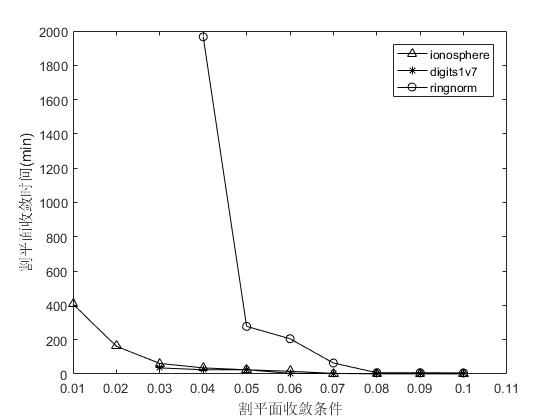
\includegraphics[width=\textwidth]{figure/time.jpg}
  \caption{MKC算法的收敛情况}
  \label{fig:time}
  \end{minipage}
  \begin{minipage}[t]{0.45\linewidth}
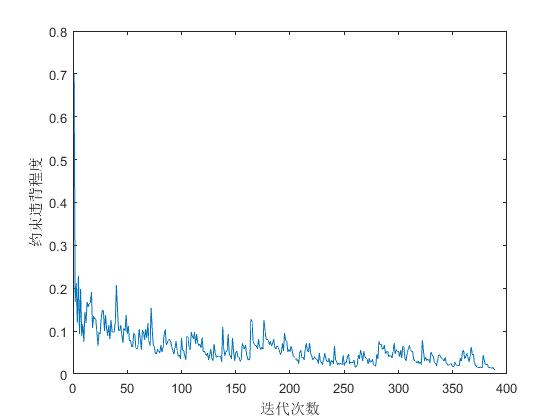
\includegraphics[width=\textwidth]{figure/ionosphere_xi.jpg}
  \caption{ionosphere割平面收敛过程}
  \label{fig:ionosphere-xi}
  \end{minipage}
  \begin{minipage}[t]{0.45\linewidth}
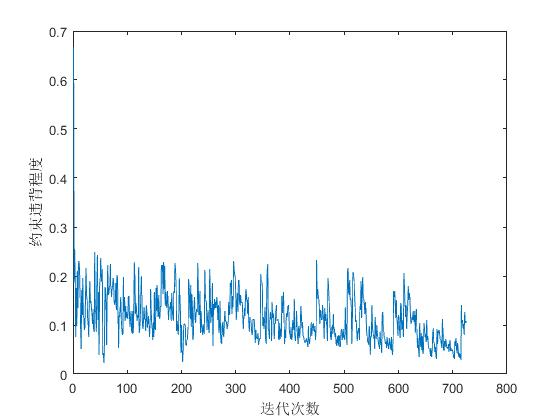
\includegraphics[width=\textwidth]{figure/digits1v7_xi.jpg}
  \caption{digits1v7割平面收敛过程}
  \label{fig:digits1v7-xi}
  \end{minipage}
  \begin{minipage}[t]{0.45\linewidth}
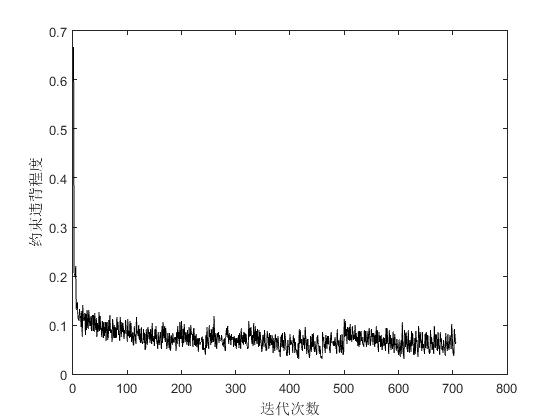
\includegraphics[width=\textwidth]{figure/ringnorm_xi.jpg}
  \caption{ringnorm割平面收敛过程}
  \label{fig:ringnorm-xi}
  \end{minipage}
\end{figure}

\section{泛化能力}
MKC采用了SVM中的间隔最大化学习策略,因此本文实验也测试了MKC在未知数据上的泛化能力。首先从总数据集上随机获取一定规模的子集作为训练数据集,剩下的数据集作为测试数据集。然后利用训练数据集学习得到MKC模型,并使用此模型在测试数据集上进行聚类。
\begin{table}[!htbp]
\caption{MKC的泛化能力(\%)}
\centering
\small
\renewcommand\arraystretch{1.5}
\begin{tabular}{|p{2cm}<{\centering}|p{2.5cm}<{\centering}|p{2.5cm}<{\centering}|}
\hline
数据 & 训练数据集 & 测试数据集 \\
\hline
digits1v7 & 99.74 & 98.92 \\
\hline
ringnorm & 87.46 & 87.19  \\
\hline
\end{tabular}
\label{tab:generalize}
\end{table} 

观察表(\ref{tab:generalize}),发现对数据集的子集进行训练得到的模型在测试数据集上也能取得较好的效果,也即泛化性能较好。受这个结果的启发,在对数据集进行学习训练过程中,若数据集规模较大,可以以一定的策略(比如随机)选择数据集的一个小的子集作为训练集,再在这个训练集上进行训练,得到的MKC模型在整个数据集上同样能得到很好的聚类效果。

\section{本章小结}
本章使用UCI上的数据集进行实验来验证MKC模型的性能,并与传统的k均值聚类和谱聚类进行比较。从前面的实验可以看出,与传统的k均值和谱聚类相比,MKC算法的聚类精度较高,较好的克服了数据集内部结构对模型聚类精度的影响。但MKC模型的训练过程需要较长的时间,并且其割平面迭代过程很不稳定,每轮割平面得到的模型进行聚类时,得到的精确度跳跃特别大,上下剧烈抖动,造成割平面收敛时得到的模型不一定是最优的,本文以迭代过程中聚类精度最高的参数作为最优模型的参数。此外,MKC算法具有较好的泛化性能,这使得MKC算法能轻松应对大规模数据集。
\chapter{结束语}
\section{本文工作小结}
本文就如何将SVM中的间隔最大化学习策略和核技巧应用到无监督的聚类学习中进行了深入研究。首先,分别从SVM的主问题和对偶问题出发,分析了SVM的学习问题,讨论了模型的构建、优化问题的推导以及二者之间的关系等问题,并研究了间隔最大化学习策略和核技巧在SVM中的应用方法。

其次,将SVM推广到无监督学习中,为无类别标记的训练数据添加一组标记,使得其经过SVM训练学习后,能得到最大的间隔,这就是最大间隔聚类MMC。MMC通过使用一些了线性约束来替换原始非凸整形规划问题的非凸约束,得到凸整形规划问题,然后再松弛其中的整形约束,从而得到最终的SDP问题,并能通过现有的半定规划工具包进行求解。但MMC在松弛约束的过程中会损失部分参数空间,并且与其它核方法一样,寻找合适的核函数是个比较困难的问题。

进一步,在MMC的基础上引入有监督和半监督学习中的多核学习的思想,使用多个核函数的非负线性组合得到新的基核,并使用此基核进行训练、学习。并针对MMC中出现的非凸整形规划问题,MKC应用割平面算法,构造一系列逐渐逼近该问题的序列,并且序列中的每个问题都可以使用CCCP求解。MKC最终能在训练数据上找到最大间隔超平面、最适当的类标记组合以及最优的核函数组合。

最后,在对MMC和MKC模型进行详细探讨之后,通过实验来验证其性能的优越性。本文使用UCI上的数据集,对MMC、MKC、k均值和谱聚类的聚类精度进行比较,并对MMC和MKC的聚类性能作出评价。

\section{进一步的工作}
本文深入分析了MMC和MKC的聚类原理以及模型推导过程,实现了间隔最大化学习策略和核技巧向聚类的推广,并引入有监督和半监督学习中的多核思想,最终实现基于间隔最大化学习策略和核技巧的多核学习聚类模型。在此基础上,本文还有以下工作可以进一步拓展和完善:
\begin{enumerate}[fullwidth,itemindent=24pt]
  \item 选用计算能更强的设备,使用更多的数据集对模型性能进行测试,以便客观的评价模型的性能。
  \item 分析MKC算法的时间复杂度和聚类精度,为MKC算法的收敛速度和聚类精度提供理论支持。
  \item 考虑多分类SVM模型,并在此基础上尝试将MKC推广为多类分类模型,再进行相关实验验证多类MKC模型的性能。
\end{enumerate}
\chapter*{致\hspace{1cm}谢}
\addcontentsline{toc}{chapter}{致谢}
时光如白驹过隙,转眼间我即将完成四年的本科生生涯。这三年多的时间见证了我的成长,一路走来,收获太多。此时此刻我的心中充满了感动,在这里我要感谢所有师长、同学和家人的指导、支持和帮助。

首先我要感谢王敏老师和东南大学的薛晖老师以及李森学长。历时半年之久的毕业设计,从最初的选题、写开题报告,到后来的初稿、定稿,都不是一帆风顺,因为她们的严格要求、督促和指导,让我顺利完成本科毕设设计。在这里我要对他们给予我的指导和帮助致以最衷心的感谢。

其次,我要感谢河海大学计算机与信息学院12级辅导员姜彬彬老师对我的教诲和关怀,以及所有授课教师的授业解惑,他们在我人生的成长道路上留下了浓墨重彩的一笔,在这里我要对他们给予我生活和学习上的帮助致以最崇高的敬意。

此外,我要感谢我的室友在这三年多的时间里给予我的关怀与帮助,是他们为我营造了积极和睦的生活环境。

最后,在我即将走出校门,踏入研究生生涯之际,我要感谢我的父母和亲人。没有他们这么多年来多我的关怀、支持和鼓励,就不会有今天的我。

仅以此文献给所有关心和帮助过我的人。

\clearpage
\addcontentsline{toc}{chapter}{参考文献}
\bibliographystyle{unsrt}
\bibliography{refference/reffer}


\includepdfset{pagecommand={\thispagestyle{plain}}}
\begin{appendix}
   \chapter*{算法源码}
\addcontentsline{toc}{chapter}{算法源码}
\noindent 本文中的MKC算法的核心Matlab代码如下:
\begin{lstlisting}[basicstyle=\small\menlo]
% 参数介绍
% data为待输入的训练数据,矩阵类型,每行表示一条训练数据,每列表示训练数据的属性
% label为训练数据的标签,列向量,元素取值为-1或1
% C为松弛参数
% d为多项式核函数的参数
% sigma为高斯核函数的参数
% epsilon为割平面过程的终止条件,这里默认为0.05
% alpha为CCCP过程的终止条件,这里默认为0.01
% best_v为在当前模型参数下,割平面过程中使得聚类精度最高的权值参数
% best_b为在当前模型参数下,割平面过程中使得聚类精度最高的偏置参数
% max_acc为在当前模型参数下的最高聚类精确度
function [ best_v, best_b, max_acc ] = mkc( data, label, C, d, sigma, epsilon, alpha )
if nargin == 5	% 设置默认值
    epsilon = 0.05;
    alpha = 0.01;
end
[m,n] = size(data);
l = m/3;  	% 类平衡约束条件
M = 3;     % 核函数个数,这里包括线性核函数、多项式核函数、高斯核函数
linear_kernel = data * data';  	% 线性核函数生成核矩阵
polynomial_kernel = (data * data'+1).^d; % 多项式核函数生成核矩阵
guass_kernel = zeros(m,m);
for i = 1:m
    for j = 1:m
	data_temp = data(i,:) - data(j,:);
	guass_kernel(i,j) = exp(-data_temp*data_temp'/(2*sigma)); 	% 高斯核函数生成核矩阵
    end
end
X = {};
X{1} = getFeature(linear_kernel);	% 根据核矩阵获取其特征
X{2} = getFeature(polynomial_kernel);	% 根据核矩阵获取其特征
X{3} = getFeature(guass_kernel);	% 根据核矩阵获取其特征
C_Omega = {};		% 保存所有最违背的约束,也即约束子集Omega
max_acc = -inf;
% 开始割平面过程,在每轮割平面中进行CCCP过程,并求解每轮CCCP中的最优化问题
while 1	% 割平面迭代过程
    v_k = ones(m,M);
    b_k = 1;
    res_temp = inf;
    while 1		% CCCP迭代过程
        cvx_begin sdp quiet		% 使用cvx优化包,一次CCCP求解过程
            cvx_solver mosek		% 使用mosek求解器
            variables betta(M) T(M) 
            variables xi(1) b(1) 
            variable v(m,M)
            minimize(0.5*sum(T)+C*xi)	% 最小化目标函数
            subject to 		% 所有约束条件
                % 基础约束
                for i=1:M
                    norm([2*v(:,i);T(i)-betta(i)]) <= T(i)+betta(i);
                    betta(i) >= 0;
                end
                sum(betta.^2) <= 1;
                xi >= 0;
                l_temp = zeros(1,m);
                for i=1:M
                    l_temp = l_temp + v(:,i)'*X{i}';
                end
                -l <= sum(l_temp+b) <= l; 
                % 由最违背约束子集Omega生成的约束条件
                if numel(C_Omega) > 0
                    z_temp = zeros(1,m);
                    for i=1:M
                        z_temp = z_temp + v_k(:,i)'*X{i}';
                    end
                    z = sign(z_temp+b_k)';
                    for i=1:numel(c_arr)
                        1/m*sum(C_Omega{i}) <= xi+1/m*((C_Omega{i}.*z)'*(l_temp+b)');
                    end
                end
        cvx_end		% 最优化问题求解完毕
        res = cvx_optval;
        % 判断是否满足CCCP迭代终止条件
        if abs((res-res_temp)/res) <= alpha
            break;
        end
        v_k = v;
        b_k = b;
        res_temp = res;
    end	% CCCP迭代终止,进入割平面过程
    temp = zeros(1,m);
    for i=1:M
        temp = temp + v(:,i)' * X{i}';
    end
    temp = (temp + b)';
    c = zeros(m,1);     % 初始化最违背约束对应的c向量
    xi_m = 0;
    for i = 1:m     % 寻找最违背的约束
        if abs(temp(i)) < 1
            c(i) = 1;
        else
            c(i) = 0;
        end
        xi_m = xi_m + c(i) * (1 - abs(temp(i)));
    end
    xi_m = xi_m / m;
    cluster = sign(temp);	% 聚类生成的样本类别标记
    acc = sum(label==cluster)/m;	% 计算聚类准确率
    if acc < 0.5		% 保证多数原则
        acc = 1 - acc;
    end
    if max_acc < acc		% 判断本次迭代的聚类准确率是否最优
        max_acc = acc;
        best_v = v_k;
        best_b = b_k;
    end
    if xi_m-xi <= epsilon	% 判断是否满足割平面过程的终止条件
        break;
    end
    % 将最违背的约束加入约束子集,再进入CCCP过程
    C_Omega{numel(C_Omega)+1} = c;
end
end

% 特征提取函数参数介绍
% K为由核函数生成的样本矩阵,也即核矩阵
% X为对核矩阵进行特征分解得到的特征向量
function [ X ] = getFeature( K )
n = length(K);
[p,x] = eig(K);
for i=1:n
    if x(i,i) < 0
        x(i,i) = 0;
    end
    x(i,i) = x(i,i)^0.5;
end
X = p * x;
end
\end{lstlisting}
   \clearpage
   \addcontentsline{toc}{chapter}{英文文献}
   \includepdf[pages=1-12]{translate/multiplekernelClustering.pdf}
   \addcontentsline{toc}{chapter}{文献翻译}
   \includepdf[pages=1-28]{translate/multiplekernelClustering中文版.pdf}
\end{appendix}


\end{document}  